\documentclass{standalone}

\usepackage{../styles/math,../styles/figures}


\usepackage{tikz}
\usetikzlibrary{shapes,arrows,matrix,positioning}

\begin{document}

\begin{tikzpicture}
  % Define block styles
  \tikzstyle{block} = [draw=black!80, thick, text width=8em, text centered, minimum height=3em, outer sep=0pt]
  \tikzstyle{sharp} = [block, rectangle, draw=white!70!black, line width=1.2mm, fill=blue!20]

  \tikzstyle{rounded} = [block, rectangle, rounded corners=5pt, line width=1.2mm, fill=green!20]
  \tikzstyle{arrow} = [thick,->,>=latex, shorten >=3pt, shorten <=3pt, draw=black!80, line width=1.5mm]

  \tikzstyle{roundedblock} = [matrix, draw=black!80, rounded corners=5pt, line width=1.2mm, fill=black!10, column sep=0.8cm, row sep=0.5cm, inner sep=2em]

  \tikzset{image/.style={above right, inner sep=0pt, outer sep=0pt}}

  % % Sharp-edge blocks
  % \node [sharp] (sharp1) at (0,0) {Sharp 1};
  % \node [sharp, right=of sharp1] (sharp2) {Sharp 2};

  % % Rounded-edge blocks
  % \node [rounded, below=of sharp2] (rounded1) {Rounded 1};
  % \node [rounded, below=of sharp1] (rounded2) {Rounded 2};

  % Main block with nested nodes (increased width, constant sub-block width)
  \node [roundedblock] (ctr) {
    \node (qp) [rounded, text width=20em, minimum height=3cm, fill=red!20] {\Huge \textbf{CONTROLLER}}; \\
  };

  \node[image, right=3cm of ctr] (sys) {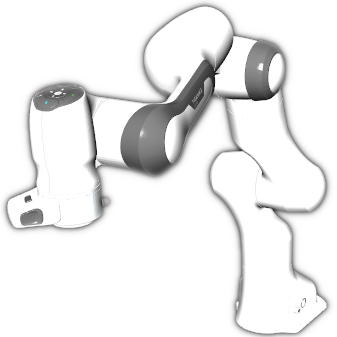
\includegraphics[scale=0.6]{images/franka_robot}};

  \node [rounded, below=3.5cm of sys, xshift=0.5cm, text width=5em, inner sep=1.5em] (fk) {\Huge \textbf{FK}};

  \node [roundedblock, below left=7cm and -5cm of qp] (ds) {
    \node (ds_trans) [rounded,  text width=18em, fill=blue!20, minimum height=4cm] {\centering \Huge \textbf{DYNAMICAL} \\ \vspace{5mm} \textbf{SYSTEM}}; \\
  };


  \node [rounded, text width=10em, inner sep=1em, below right=-2.7cm and 3.5cm of ds] (exp_map) {\Huge $\text{Exp}\rbr{\sbr{\boldsymbol{\theta}}_{\times}}$};

  % Arrows
  \draw [arrow] (ctr) -- (sys) node[midway, above] {\Huge $\boldsymbol{\tau}$};
  \draw [arrow] ([xshift=1.0cm]sys.south) -- ([xshift=0.5cm]fk.north) node[pos=0.25, right] {\Huge $\mathbf{q}$};
  \draw [arrow] (sys.south) -- ([xshift=-0.5cm]fk.north);
  \draw [arrow] ([xshift=1.0cm]sys.south) -- ++(0, -2cm) -| ([xshift=-1.0cm]ctr.south);
  \draw [arrow] (sys.south) -- ++(0,-1.5cm) node[pos=0.5, left] {\Huge $\mathbf{\dot{q}}$} -| ([xshift=1.0cm]ctr.south); % [xshift=-2cm,yshift=+3pt]fk.north
  \draw [arrow] ([xshift=-0.5cm]fk.south) |- ([yshift=1.0cm]ds.east) node[pos=0.93, above] {\Huge $\v{x}, \td{\v x}$};
  \draw [arrow] ([xshift=0.5cm]fk.south) |- (exp_map.east) node[pos=0.83, below] {\Huge $\boldsymbol{\theta}, \dot{\boldsymbol{\theta}}$};
  \draw [arrow] (exp_map.west) -- ([yshift=-1.0cm]ds.east) node[pos=0.5, below] {\Huge $\m{R}, \td{\m R}$};

  \draw [arrow] ([yshift=1.0cm]ds.west) -- ++(-2.5cm, 0) |- ([yshift=-0.5cm]ctr.west) node[pos=0.87, below] {\Huge $\mathbf{\dot{x}}, \mathbf{\ddot{x}}$};
  \draw [arrow] ([yshift=-1.0cm]ds.west) -- ++(-3cm, 0) |- ([yshift=0.5cm]ctr.west) node[pos=0.87, above] {\Huge $\boldsymbol{\omega}, \dot{\boldsymbol{\omega}}$};
\end{tikzpicture}

\end{document}